\chapter{GBT IF System}\label{appendix:if}

In this appendix we provide a general outline of the \gls{GBT} \gls{IFsys}.
Figures~\ref{fig:ifpath} and ~\ref{fig:ifsys} give a simplified overview
of the \gls{GBT} \gls{IFpath} and will guide our discussion.  We will
not cover \gls{MUSTANG} as it is a direct detection system.  Note that during
each frequency mix, each polarization pair is mixed with a signal from the
same synthesizer. All synthesizers are locked to our H-maser frequency standard.

\begin{figure}[!h]
\begin{center}
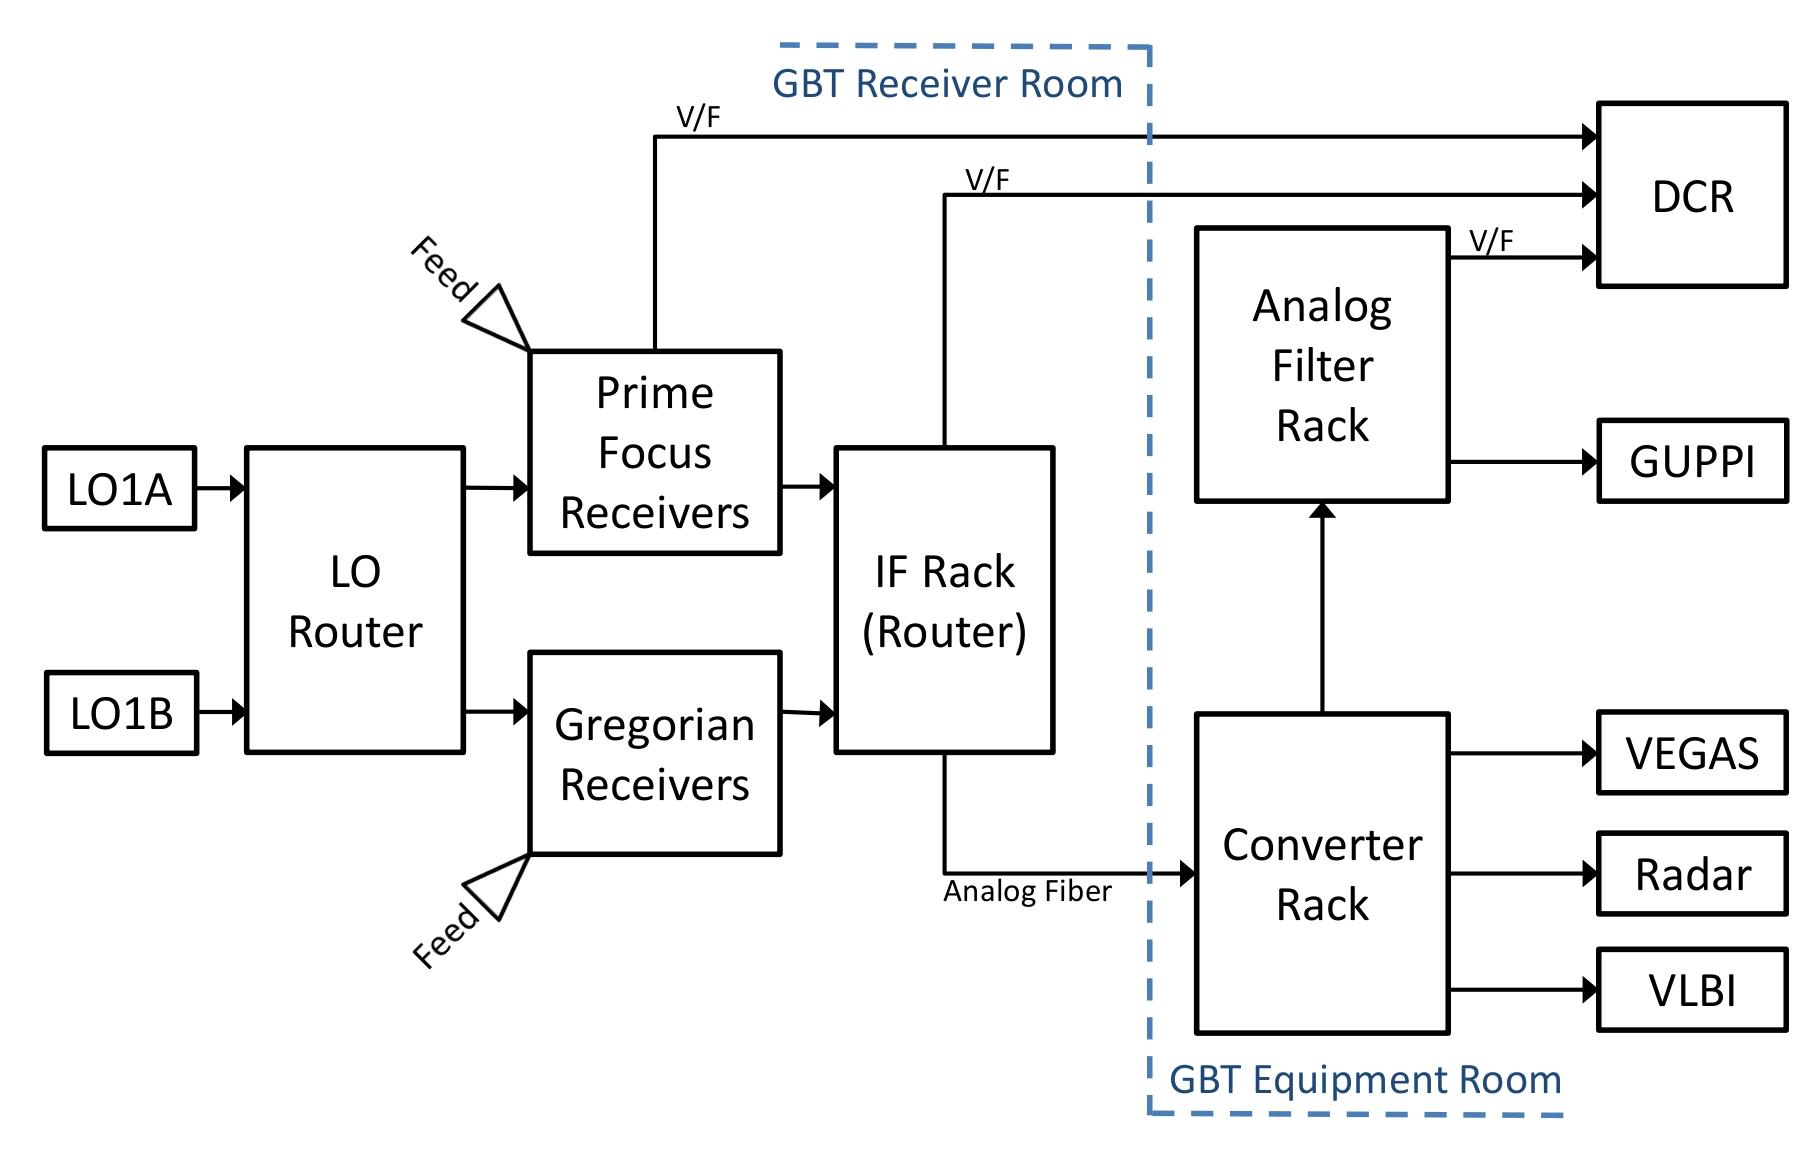
\includegraphics[width=\linewidth]{GBTifSys.jpg}
\caption[GBT IF system routing]
{A simplified flow diagram of the \gls{GBT} \gls{IFsys} routing.
\label{fig:ifpath}
}
\end{center}
\end{figure}

\begin{figure}[!h]
\begin{center}
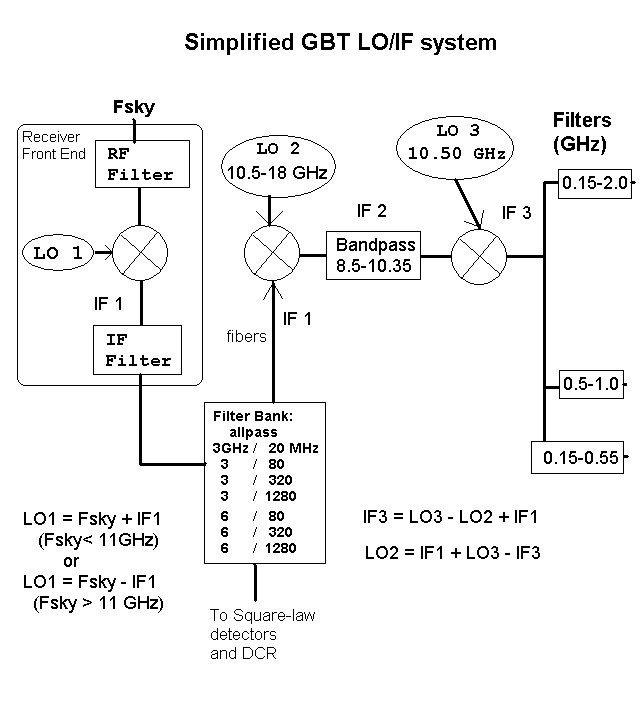
\includegraphics[width=0.85\linewidth]{IFsystemn.jpg}
\caption[GBT IF system flow chart]
{A simplified flow chart of the \gls{GBT} \gls{IFsys}.
\label{fig:ifsys}
}
\end{center}
\end{figure}

\newpage
\section{From the Receiver to the IF Rack}

The frequency that is observed is given by ${\rm F_{sky}}$.  Within the receiver the
detected signal at ${\rm F_{sky}}$ is mixed with the \gls{LOone} signal.  The
\gls{LOone} frequency is derived from a synthesizer and can vary in time when
Doppler tracking the velocity of a spectral line.  The result of the mixing of
${\rm F_{sky}}$ and \gls{LOone} is the \gls{IF} frequency, IF~1. The typical IF~1
center frequencies are 1080, 3000 and 6000~MHz. Filters limit the bandwidth in
the receivers both before and after the \gls{LOone} mix.  There are also filters
in the \gls{IFRack} that limit the bandwidth.  The resulting allowed bandwidths
are 20, 80, 320, 1280~MHz and \dq{All Pass} (i.e. no filtering other than the
response of the receiver).  

Before the \gls{IFRack} each signal is split into two (single beam receivers only)
copies of the original signal. Each signal in the \gls{IFRack} is detected and then
sent to the \gls{DCR} (as used during pointing and focus observations).  Each signal
is also sent as an analog signal over optical fiber to the Jansky Lab to the \gls{CRRack}.

\newpage
\section{From the Converter Rack to the Backend}

When the signal reaches the \gls{CRRack} it is split into four separate copies.
This allows up to eight different copies of the received signal for single beam
receivers and four copies of each received signal for dual beam receivers.  

In the \gls{CRRack} the signal is mixed with the \gls{LOtwo} signal.  Each copy
of the signal can be mixed with a different \gls{LOtwo} since there are eight
different \gls{LOtwo} synthesizers.  The resultant signals are then sent through
a filter to make sure it has a bandpass of no more than 1.85~GHz.  A final mix
with a fixed frequency of 10.5~GHz then gets the signal within the input band-passes
of the backends.  There is a final set of filters that ensures the signal has the 
correct bandwidth for the backend.

\begin{figure}[!h]
\begin{center}
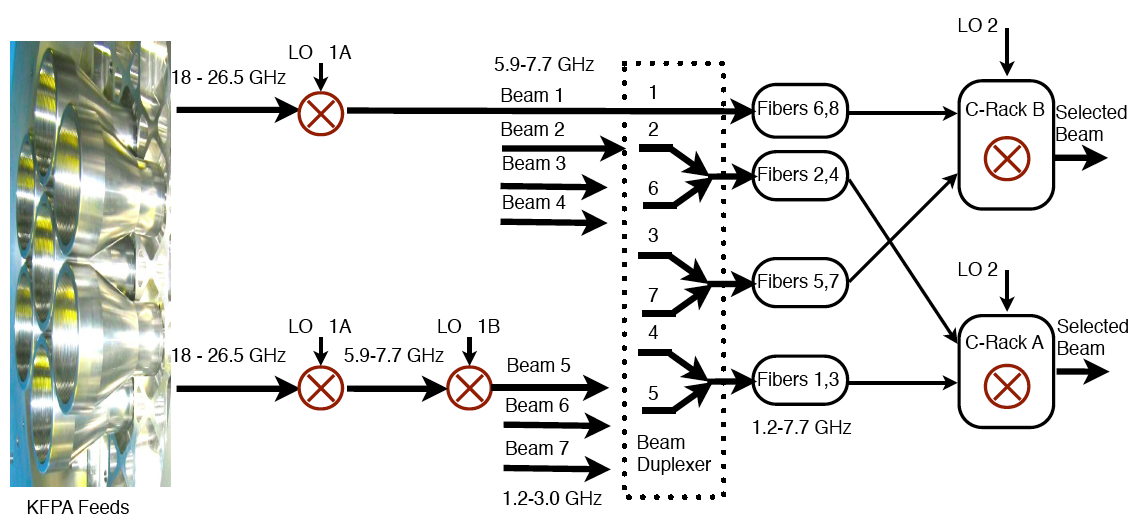
\includegraphics[width=\linewidth]{SimpleKfpaIf.png}
\caption[KFPA IF system chart]
{A simplified KFPA diagram showing the combination of beams onto fiber modems
and their selection in the Converter Rack Modules A and B.
\label{fig:kfpaIf}
}
\end{center}
\end{figure}

\section{KFPA Combined IF}\label{sec:KfpaIF}

The KFPA receiver, with 7 beams, is the first GBT receiver with more \gls{IF}
signals than there are Optical Fibers from the GBT to the Jansky Lab. In order to
bring the \gls{IF} signals to the control room, pairs of signals from different
beams were duplexed on single fibers. The signal combination was accomplished by
an analog addition of the \glspl{IF} of pairs of beams.   Beams 1,2,3 and 4
have \gls{IF} signals centers at 6800 MHz. The \gls{IF} signals from beams
5, 6 and 7 are down converted to 2100 MHz center frequency.  Beam 2 is paired
with 6, beam 3 with 7 and beam 4 with 5 (See Figure \ref{fig:kfpaIf}).

At the \gls{CRRack} one of the two beams is selected by appropriately setting the
converter rack LO frequency.  Beams 2, 4, 5 and 6 are routed to \gls{CRRack} A and
beams 1, 3 and 7  to \gls{CRRack} B.  This constrains certain multi-beam observing
modes, as is described in Chapter~\ref{chap:kfpa}.

%Note that each GBT receiver has a maximum frequency offset between spectral 
%windows, set by band pass filters in the IF path.
%For the \gls{KFPA}, due to the dual use of individual optical fibers, there are
%strong constraints on the frequency separation of the individual spectral windows.
%The maximum spectral window separation is 1.8 GHz and the maximum offset 
%between the spectral window and the Doppler tracking frequency is 1.0 GHz.
%See Appendix~A for more details on the syntax 
%for describing spectral windows.




%++++++++++++++++++++++++++++++++++++++++++++++++++++++++++++++++++++++++++++